\documentclass{article}
\usepackage{amsmath}
\usepackage{float}
\usepackage{graphicx, wrapfig} 

% \usepackage{graphicx}

\title{Theoretical mechanics. Homework 1}
\author{Ekaterina Mozhegova}
\date{\today}

\begin{document}
\maketitle

\section{Task 1}

\subsection{Tools}

Python (Matplotlib, scipy, sympy)

\subsection{Link to the simulation}

https://colab.research.google.com/drive/18xTHbIfrOZOSFk18J3NwOZv4AvnBLmiQ?usp=sharing

\subsection{Task description}
You should find:
\begin{enumerate}
    \item Simulate the move of \(\vec{O}\) for \( t = [0..10] \).
    \begin{align*}
        \vec{O} &= \begin{bmatrix} x \\ y \end{bmatrix} = \begin{bmatrix} 3 \cos(2t) \cos(t) + 0.82 \\ 3 \cos(2t) \sin(t) + 0.82 \end{bmatrix}
    \end{align*}
    \item Find and draw plots \( v \), \( a \), \( a_n \), \( a_{\tau} \), \( \kappa \) (Osculating circle) with respect to \( t \); 
    \item Find \( y(x) \), \( \vec{v} \), \( \vec{a} \), \( \vec{a}_n \), \( \vec{a}_{\tau} \) and show it on the simulation.
\end{enumerate}

\subsection{Task explanation}
1) Projections of  velocity on x and y are found as $\dot x$ and $\dot y$ respectively, then the total velocity is found by the following formula: 
\(v = \sqrt{v_x^2 + v_y^2}\).

2) Projections of the acceleration are $\ddot{x}$ and $\ddot{y}$. 

Tangential acceleration $a_\tau = \dfrac{\vec{a} \cdot \vec{v}}{|\vec{v}|}$. 
Since $a = \sqrt{a_\tau^2 + a_n^2}$, the normal acceleration $a_n$ can be found as $a_n = \sqrt{a^2 - a_\tau^2} = \sqrt{a_x^2 + a_y^2 - a_\tau^2}$.

3) The curvature (K) of a curve can be found as a cross product of the velocity and acceleration vectors over the cube of the magnitude of the velocity vector: 

$K = \dfrac{\| \mathbf{r}'(t) \|^3}{\| \mathbf{r}'(t) \times \mathbf{r}''(t) \|}$

$K = \dfrac{\left| v_x a_y - v_y a_x \right|}{v^3}$

4) To find y(x), we can apply a method of interpolation for the generated points x and y. However, the function represented by the provided parametric equation does not constitute a function in the algebraic sense, as it lacks a strict one-to-one correspondence between x and y values. For greater precision, the curve should be treated as a piecewise function.
To improve the result we can consider the following marked approximate regions where the leaves might be located.

\begin{figure}[H]
    \centering
    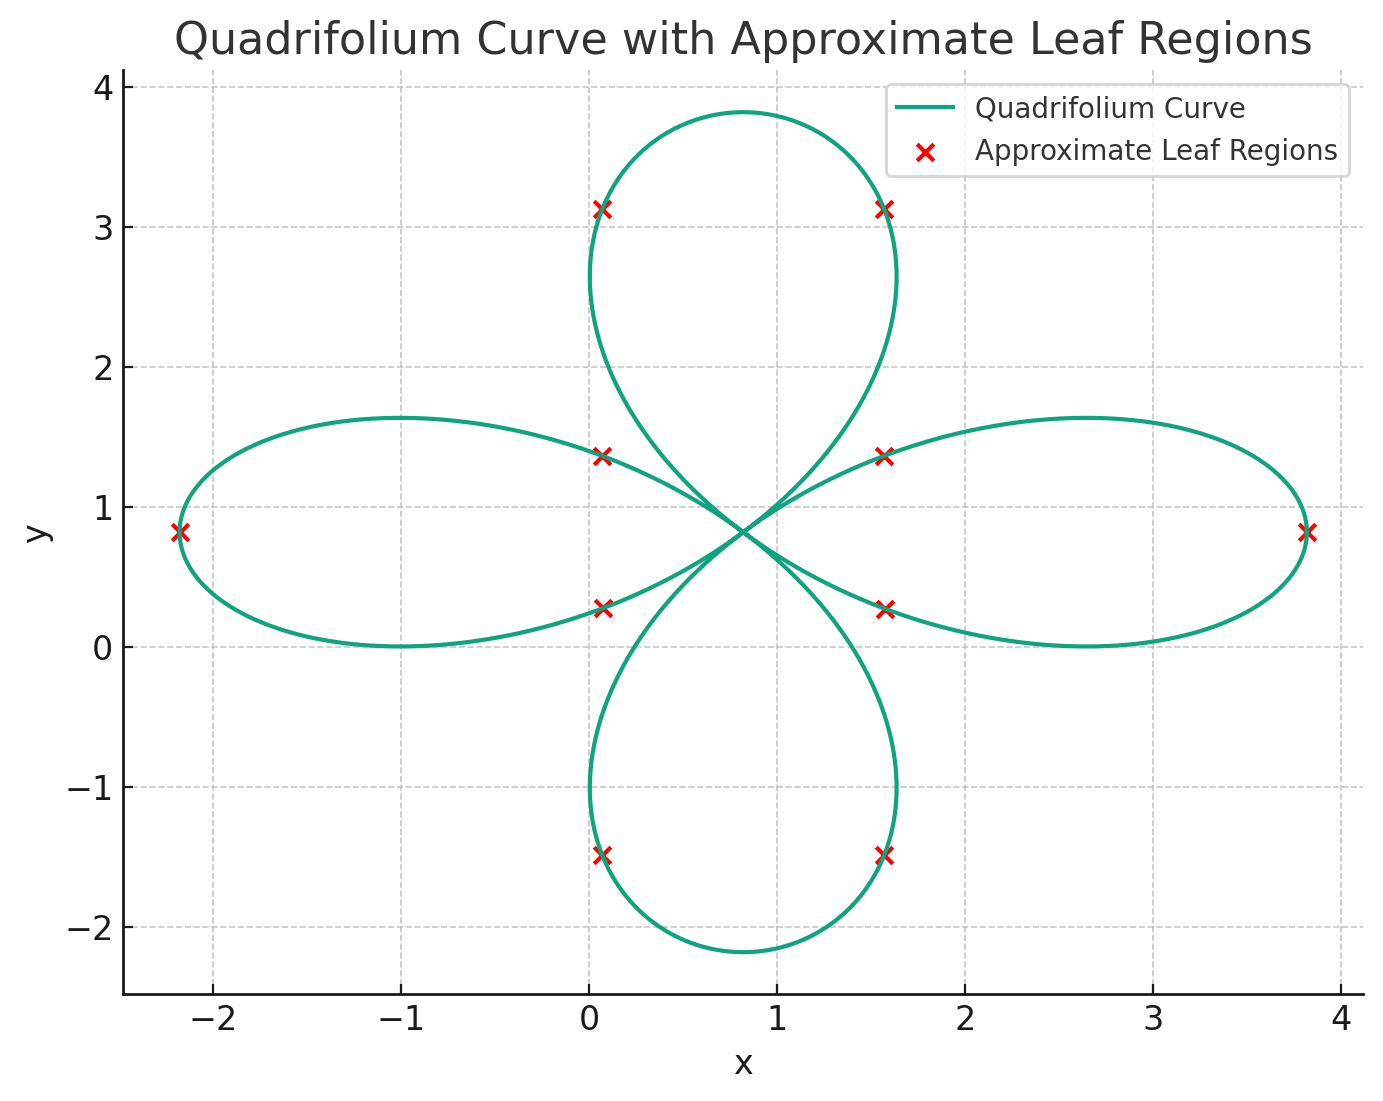
\includegraphics[width=0.5\textwidth]{quadrifollium.png}
\end{figure}


\subsection{Plots}

\begin{figure}[H]
    \centering
    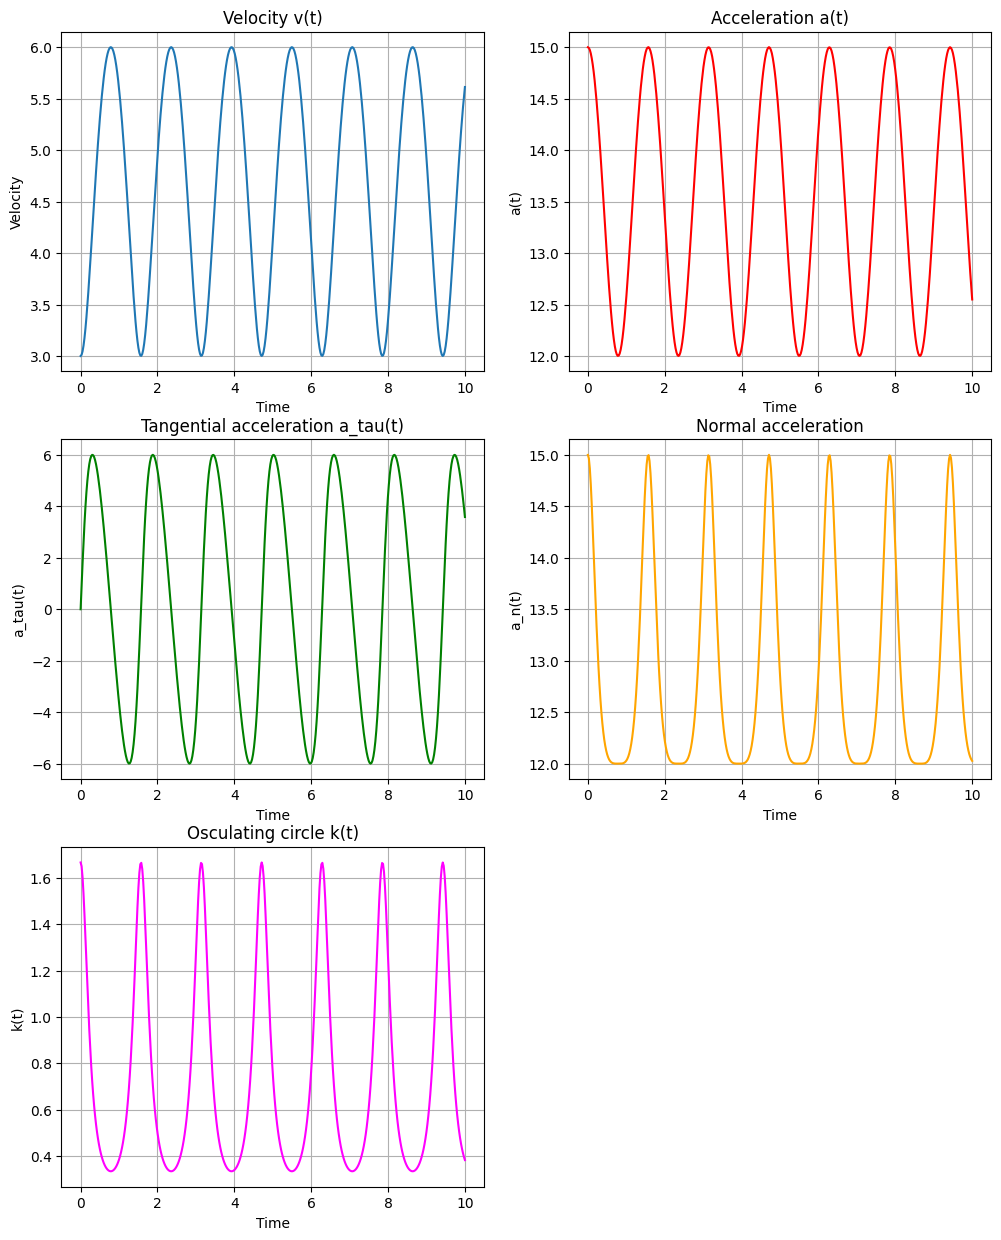
\includegraphics[width=0.9\textwidth]{Task1.png}
\end{figure}

\subsection{Screenshots from simulation}

Several screenshots, in some interesting positions. Example: parabola —
midway of left branch, root, somewhere in right branch.


\section{Task 2}

\subsection{Tools used for the task}
GeoGebra

\subsection{Link to the simulation}
https://www.geogebra.org/calculator/jveychw3

\subsection{Task description}

You should solve the task, till the M point travels s:

1. Simulate this mechanism (obtain all positions of
bodies 1, 2, 3)

2. Velocity for M(draw plots for magnitudes and
show vectors on simulation);

3. Accelerations (tangent, normal, overall) for
M(draw plots for magnitudes and show vectors
on simulation);

4. Draw plots of angular velocities for 2, 3 bodies.

% If R2 = 40, r2 = 30, R{3} = 15, x = x(t) = 3 + 80t^2 , sM = 0, 5.

If \( R_2 = 40, r_2 = 30, R_3 = 15, x = x(t) = 3 + 80t^2 \), and \( s_M = 0.5 \).

\begin{figure}[H]
    \centering
    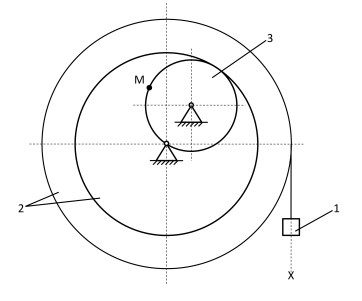
\includegraphics[width=0.5\textwidth]{Task2.png}
    \caption{Task 2\label{Task 2}}
\end{figure}

\subsection{Task explanation}

To implement a simulation, it is necessary to know the time interval. Find t by the following way:

1) \(x(t) = 3 + 80t^2 \)

\( v(x) = \dot x = 160t\)

$\omega = \dfrac{160t}{40} = 4t$

$\omega_2 = 4t$

Linear velocities of the ineer part of the big wheel is equal to the linear velocity of the  small 
wheel.

$\omega_2 r_2 = \omega_3 R_3 $

$v_3 = \omega_3 R_3 = \omega_2 r_2$

\( s = \int v_3(t) dt = 5\)

\( s = \int \omega_3 R_3 dt = \int \omega_2 r_2 dt  = \int 4t r_2 dt = 2t^2 r_2 \Rightarrow t = \sqrt{\dfrac{s}{4 r_2}} \approx 0.28868\)  


Once you found time interval t, the simulated objects can be represented as functions of t, which are moving in a way corresponding
the time change.

\subsection{Plots}
5. Plots. Put needed plots. Don’t forget to make an appropriate title, legend, and axes description.
\subsection{Screenshots from simulation}

Several screenshots, in some interesting positions. Example: parabola —
midway of left branch, root, somewhere in right branch.


\section{Task 3}

\subsection{Link to the simulation}

https://www.geogebra.org/calculator/erfh2pn8

\subsection{Task description}

You should find:

1. Simulate this mechanism (obtain all positions.)
(xi (t), yi (t), where i is A, B, C point)

2. Velocities for B, C (draw plots for magnitudes and
show vectors on simulation);

3. Accelerations for B and C (draw plots for
magnitudes and show vectors on simulation);

4. Draw a plot of angular velocity of body BA.

$y_A(t) = 22.5 + \sin(5\pi t)$, where $t \in [0, 10]$ sec; AB = 45, AC = 30.

\begin{figure}[H]
    \centering
    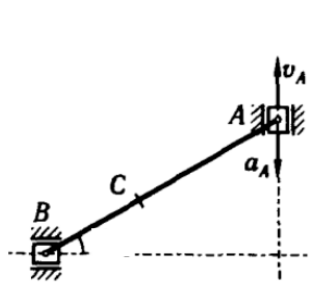
\includegraphics[width=0.35\textwidth]{Task3.png}
    \caption{Task 3}
\end{figure}


\subsection{Task explanation}

1) We can find the law of motion for the body B from the right triangle by the Pythagorean's theorem. 
$x_{b}(t) = \sqrt{AB^{2} - (y_{a}(t))^{2}}$.

Velocity $u_b = \dot x_{b}(t)$.

2) To find the velocity at point C, first we need to find the instantaneous center of zero velocity $I_c$.

$I_c$ lies at the point of intersection of lines perpendicular to the vectors of A's and B's velocities.


\begin{figure}
    \centering
    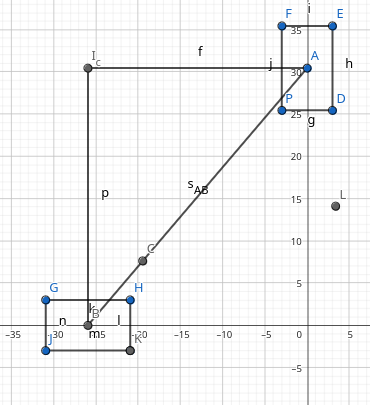
\includegraphics[width=0.5\textwidth]{Task3_mechanism.png}
    \caption{Detect Ic}
\end{figure} 

Then, \( v_c = \omega_\text{AB} \cdot CI_c\)

3) Let's find $\omega_\text{AB}$. 

$\omega_\text{AB} = \dfrac{v_a}{AB}$, where $v_a = \dot{y}_a(t)$.
\subsection{Plots}
5. Plots. Put needed plots. Don’t forget to make an appropriate title, legend, and axes description.
\subsection{Screenshots from simulation}

Several screenshots, in some interesting psositions. Example: parabola —
midway of left branch, root, somewhere in right branch.


\end{document}